% main.tex
\documentclass{scrarticle}
% 00_preamble.tex

\usepackage[authordate, backend=biber, natbib=true]{biblatex-chicago}
\addbibresource{bibliography.bib} % my bib file

\usepackage[T1]{fontenc}
\usepackage[utf8]{inputenc}
\usepackage[most]{tcolorbox}
\usepackage[noframe]{showframe}
\usepackage{mwe}
\usepackage{scrlayer-scrpage}
\usepackage{hyphenat}
\usepackage[english]{babel}
\usepackage{blindtext}
\usepackage{fontaxes}
\usepackage{hyperref}
\usepackage[bottom,splitrule,hang,flushmargin]{footmisc}

\usepackage[
    protrusion=true,
    expansion=true,
    spacing=true,
    tracking=true,
    kerning=true
]{microtype}

\KOMAoptions{
    paper=a5,
    fontsize=12pt,
    egregdoesnotlikesansseriftitles,
    headings=small,
    headings=optiontohead,
    BCOR=5mm,
    DIV=14,
    parskip=false,
    footnotes=multiple,
    twoside=true,
}

% HEADER
\setlength{\headsep}{1\baselineskip}
\setlength{\headheight}{3\baselineskip}
\setkomafont{pagehead}{\normalfont}
%%% \*head[<for 'plain' page>]{<for 'scrheadings' page>}
\ohead[\lsstyle NUMBER~\liningfigures{\Number}]{}
\chead[\lsstyle\MakeUppercase{\Month}~\liningfigures{\Year}]{\small\scshape\MakeLowercase{\Journal}}
\ihead[\lsstyle VOLUME~\liningfigures{\Volume}]{}
%%% Fill in the blanks
\lehead{\small\thepage}
\rohead{\small\liningfigures{\thepage}}
\lohead{\small\Year]}
\rehead{\small[Vol.~\Volume}
\cohead{\small\scshape\MakeLowercase{\Title}}

% FOOTER and FOOTNOTE
\setlength{\footskip}{1.5\baselineskip}
\setkomafont{pagefoot}{\normalfont}
%%% \*foot[<for 'plain' page>]{<for 'scrheadings' page>}
\ofoot[\small\liningfigures{\thepage}]{}
\cfoot[]{}
\ifoot[]{}
\setfootnoterule[]{\textwidth}

% FONT
\usepackage[osf]{Baskervaldx}

% SECTION HEADINGS
\setcounter{secnumdepth}{1}
\let\raggedsection\centering
\renewcommand{\thesection}{\Roman{section}} 
\renewcommand\sectionformat{\liningfigures{\thesection}.\enskip}
\renewcommand{\thesubsection}{\thesection.\Roman{subsection}}
\renewcommand\subsectionformat{\thesubsection.\enskip}

\setkomafont{section}{\bfseries}
\RedeclareSectionCommand[
  %runin=false,
  afterindent=false,
  beforeskip=1\baselineskip,
  afterskip=.25\baselineskip]{section}

\setkomafont{subsection}{\normalfont\itshape}
\RedeclareSectionCommand[
  %runin=false,
  afterindent=false,
  beforeskip=1\baselineskip,
  afterskip=.25\baselineskip]{subsection}

\RedeclareSectionCommand[
  %runin=false,
  afterindent=false,
  beforeskip=.5\baselineskip,
  afterskip=.25\baselineskip]{subsubsection}
  
\RedeclareSectionCommand[
  runin=true,
  %afterindent=false,
  beforeskip=.5\baselineskip,
  afterskip=1em]{paragraph}

\RedeclareSectionCommand[
  runin=true,
  %afterindent=false,
  beforeskip=.5\baselineskip,
  afterskip=1em]{subparagraph}

% LETTRINE
\usepackage{lettrine}
\setlength{\emergencystretch}{2pt}
\def\drop #1#2 {% note the space before {
  \lettrine[lines=2,loversize=0.1,nindent=2pt]{#1}{#2} % a trailing space
}

\raggedbottom


% Computer Code Styleguide. 

\usepackage{listings}
\usepackage{xcolor}

% Define more subdued colors or remove colors altogether
\definecolor{commentcolor}{rgb}{0.5,0.5,0.5} % Gray for comments
\definecolor{backcolour}{rgb}{0.95,0.95,0.95} % Very light gray background, or consider removing the background color entirely

% Setup the listings package for a professional, academic style
\lstdefinestyle{hlrstyle}{
    backgroundcolor=\color{white},   % No background color for a clean look
    commentstyle=\color{commentcolor},
    keywordstyle=\bfseries,          % Bold for keywords, no color
    numberstyle=\tiny\color{black},  % Line numbers in black
    stringstyle=\ttfamily,           % Typewriter font for strings, no color
    basicstyle=\footnotesize\ttfamily, % Typewriter font
    breakatwhitespace=true,         
    breaklines=true,                 
    captionpos=b,                    
    keepspaces=true,                 
    numbers=left,                    
    numbersep=5pt,                  
    showspaces=false,                
    showstringspaces=false,
    showtabs=false,                  
    tabsize=2
}

\lstset{style=hlrstyle}

% 01_metadata.tex
% this .tex file vcovers everything from the heading down to the keyterms and footnaotes on the first page. the rest is managed at the main.tex file.

\newcommand{\Journal}{Technical Documentation}
\newcommand{\Year}{2024}
\newcommand{\Month}{May}

\newcommand{\Volume}{I}
    \newcommand{\vol}{Vol. ~\Volume}
    \newcommand{\Vol}{VOLUME~\Volume}

\newcommand{\Number}{I}
\newcommand{\TITLE}{Brass Bot : Technological Framework for Collecting Spent Cartridges}
\newcommand{\Title}{Brass Bot}
\newcommand{\TitleFoot}{\footnote[2]{Submission for \href{https://courses.dce.harvard.edu/?details&srcdb=202403&crn=34560}{DGMD $E-17$} Spring Academic Term of 2024.}}

\newcommand{\AUTHOR}{LopezGarcia, G. Ross, D. Weinberg, C.}
\newcommand{\AuthorFoot}{\footnote[1]{Grigori LopezGarcia ALM, Donald Ross ALB, Corbett Weinberg ALB}}

\newcommand{\ABSTRACT}{This project professes the challenge of designing and prototyping an autonomous device that will collect the spent cartridges that have already been ejected from a firearm and are on the floor of a firing range.

Two distinct prototypes were developed one by Grigori LopezGarcia, the seconded by Corbett Weinberg. These prototypes were designed considering the unique constraints posed by remote collaboration and geographical dispersion of a team member. Through iterative design, integration of feedback from multiple hardware tests, the project encapsulates -- working prototypes that were a focused designed on the physical hardware. Through its triumph's and failures the difficulty of the hardware process. For better, or for worse, no simulators were used in the creation of this robot.}

\newcommand{\KEYWORDS} {Three Dimensional Printing, Autonomous Robotics, Firearm-Safety, Innovative Technologies, Material Recovery, Python}
\begin{document}
\setcounter{page}{000}
% 02_title.tex

% this file  will be added and used to creat the white space gaps 
\thispagestyle{plain}
\renewcommand*{\thefootnote}{\fnsymbol{footnote}}

\begin{tcolorbox}[width=\textwidth,center upper, fontupper=\center\LARGE,sharp corners,colframe=black,colback=white]
    {\scshape\textls[225]{\MakeUppercase{\Journal}}}
\end{tcolorbox}
\vspace{2\baselineskip}

\begin{raggedright}
    \begin{addmargin}[0em]{3em}
        {\noindent\large\MakeUppercase{\TITLE}\TitleFoot}
    \end{addmargin}
\end{raggedright}

\vspace{0.5\baselineskip}

\begin{addmargin}[1em]{0em}
    {\noindent\large\textit{\AUTHOR}\AuthorFoot}
\end{addmargin}

\vspace{0.5\baselineskip}

\begin{addmargin}[2em]{2em}
    {\noindent\small\fontsize{11}{13}\selectfont\ABSTRACT\par}
    {\vspace{0.5\baselineskip}}
    {\noindent\small\itshape\fontsize{11}{13}\selectfont{Keywords:~\KEYWORDS}\par}
\end{addmargin}

\vspace{1\baselineskip}

\pagestyle{scrheadings}
\renewcommand*{\thefootnote}{\arabic{footnote}}
\setcounter{footnote}{0}
%%% from this comment down we can start to write code taht will influence how our paper will look... the abstract is afterall the last thing we would write. 
\drop This documentation discusses the challenges: 'practical and academic' work done for the final project\ldots We go through the lens taken for the project, a guide of our production process, the hardware and software used, our results, and the continued.  
\section{Preface}
Prototyping of the two autonomous devices that are designed to collect spent brass\footnote{ejected firearm cartridges} in an indoor professional range of local, county, or state police officers.\footnote{{specifically United States Police Officers}} The remote nature of this courses' iteration, and a classmates geographic skisim from Cambridge - Massachusetts and necessitated the creation of separate hardware prototypes. This complicated our work but it did not over-engineer it. It gave us the abiltiy to replicate the difficulties of working with a scattered team across the country with different hardware.   

\section{Background}
\subsection{ Cops, Engineers, and Lobbyist}
LopezGarcia$'$s is the originator of the project -- His professional use of firearms brought regulated material into aproject that forced Ross and Weinberg to familiarize themselves with Massachusetts firearms regulations and creating alternatives for testing a robot that is supposed to use ammunition in a highly regulated and professional environment-- this is to say we used 3d printed stand ins for spent cartridges. Ross held to the majority of the bureaucratic administrative tasks and supervised the video production projects. Weinberg brought extensive engineering and fabrication experience, fabricating. 

\subsection{Starting with a Problem}
LopezGarcia identified the practicality of automating spent cartridges in a professional and sporting environment.\footnote{A single day of firearm training in a Police department can eject thousands of spent cartridges onto the gun-range.}
We began by using the legal patent as academic inspiration for a device that is able to collect spent brass.\footnote{AmmoUP LLC, ``Device for Collecting Spent Cartridges,'' U.S. Patent No US-20150264865-A1, 2015. Available online: \url{https://ppubs.uspto.gov/dirsearch-public/print/downloadPdf/20150264865}} Due to this inspiration, two distinct robot prototypes were created: `Roberto,' by LopezGarcia, and `Brassbot,' by Weinberg. Additionally, the commercial product by AmmoUp, LLC, started our design.\footnote{AmmoUp, LLC, ``Products for Rifle and Pistol Brass Collection,'' 2024. Accessed April 1st, 2024. \url{https://ammoupusa.com/product-cat/products/rifle-and-pistol-brass/}} Originally designed to pick up nuts, it has been sold and adapted to collect brass bullet casings professionally by the Delaware Police Department and multiple Delaware private firearms clubs. The project's goal was to assess the feasibility of automating the spent brass.


\section{Methodology}
In this section we expand on the hardware production of  the prototypes. The manufacturing the devices and the hardware used. We will discuss software components in software in Section {\textbf{IV. Computer Software}}. See Figure \ref{fig:img7299} and Figure \ref{Figure 4} for the assembled prototypes. 

%%%Gargia's Robot
\subsection{Duck Tape and Tupperware}
LopezGarcia$'$s 1$^{st}$ prototype, was a front wheel drive mounted onto a $20x20$ extruded aluminum frame taped with a transparent Tupperware enclosure, and 6.5' hoverboard wheels on front and caster wheels at the Tupperware's rear. Each of the four wheels were independently controlled by its ESC and managed by a Pixhawk controller stashed inside the Tupperware. Two problems arose from the Tupperware prototype. While justifying separate ESCs for fine control and fiscal budgeting was undermined by the wheels' fragile exterior and interior. A necessity for higher-quality ESCs, the Tupperware's crosswired enclosure, GPS, compass readings, and persistent trouble with hoverboard wheels and ESCs culminating in the failure of an ESC and a potential risk of damage to the entire micro controller setup. For image of the device see Figure \ref{fig:untitled1}.


\begin{figure}[h]
  \centering
  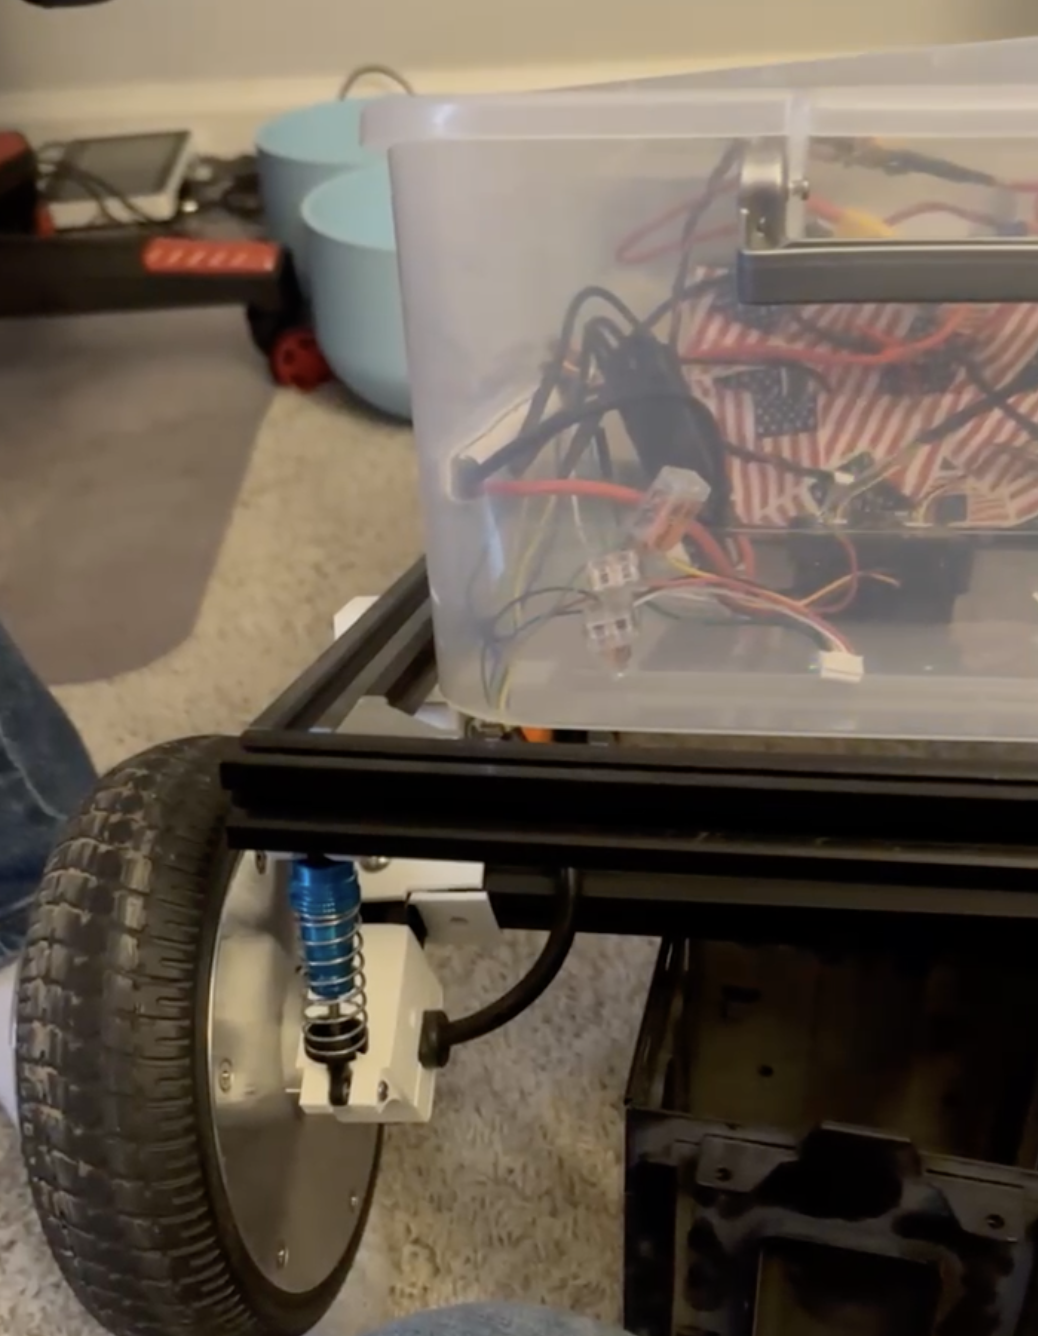
\includegraphics[width=0.5\textwidth]{Untitled.png}
  \caption{A photo of GrigorLopez's Tumpperware prototype$'$s rear caster wheels.}
  \label{fig:untitled1}
\end{figure}

The $2^{nd}$ version uses a steel RC car chassis, $1/10$ scale frame, a dramatic improvement from the previous Prototype. The transition to the RC chassis necessitated component replacement, and the calibration process was extensive. This chassis achieved success limited autonomous functionality using Mission Planner as can be seen below. 

Or see the Figure \ref{fig:img7299}. 

\begin{figure}[h]
  \centering
  \includegraphics[width=0.5\textwidth]{IMG_7299.png}
  \caption{The seconded prototype on the RC Chasis}
  \label{fig:img7299}
\end{figure}

Roberto is an autonomous rover designed to navigate and complete missions in a flat-range environment, preferably an indoor or outdoor range with a flat surface like asphalt. This project aims to create a reliable and efficient rover capable of traveling between waypoints while avoiding obstacles.

\subsection{The Tupperware Rover}
The first prototypes' unqiue pieces of hardware that were not used in the second robot were:
\begin{itemize}
    \item The hoverboard wheels required a specific, expensive ESC, and two cheap ESCs were burned out during testing.
    \item The components were haphazardly placed inside the container, resulting in a messy wiring situation.
\end{itemize}

\subsection{Prototype 2: RC Chassis-Based Rover (Roberto)}
For the second iteration, an RC chassis was used as the base for Roberto, the Major enhanced purchases:

\begin{itemize}
    \item \textbf{Chassis}: INJORA RC Frame Chassis. 
    \item \textbf{Servo}: 25KG Digital Servo High Torque for precise control. 
    \item \textbf{ESC}: GoolRC 60A Brushed ESC for reliable power management. 
    \item \textbf{Computational Control}: Raspberry Pi 4 B and Pixhawk4 reused from the $1^{st}$ prototype for advanced control and navigation. 
\end{itemize}

\subsection{Assembly of the Second Prototype}
Before assembling Roberto, it is crucial to format and configure the Raspberry Pi. This preparation allows for remote access via SSH, eliminating the need for physical SD card access post-assembly. The setup involves downloading the Raspberry Pi OS, writing it to the SD card, and performing initial configurations including Wi-Fi and SSH setup.

\subsubsection{Chassis Assembly}
The RC car chassis forms the base of Roberto. Assembly varies by model; our INJORA RC Frame Chassis required manual wheel installation, emphasizing the importance of secure attachments for robust navigation.

\subsubsection{Brushed ESC and Motor Connection}
Connecting the Electronic Speed Controller (ESC) to the motor involves precise wiring—positive, negative, and signal lines must be securely connected and insulated to prevent electrical faults.

\subsubsection{Servo Installation}
The servo, critical for steering, is mounted on the front frame. Correct installation is crucial for accurate navigation, requiring careful alignment and calibration.

\subsubsection{LiPo Battery Connection}
The LiPo battery is attached to the chassis, ensuring secure mounting and correct polarity connections.

\subsubsection{RC Receiver and Controller Setup}
The RC receiver is paired with the Flysky controller, establishing manual control essential for initial testing and troubleshooting.

\subsubsection{GPS Module Assembly}
The GPS module is mounted on the chassis with the orientation marker pointing forward, critical for accurate positional data.

\subsubsection{Pixhawk and Raspberry Pi Integration}
Integration of the Pixhawk flight controller with the Raspberry Pi involves detailed wiring and configuration to ensure effective communication between navigation components and the control software.

\subsubsection{Telemetry Module and Mission Planner}
The telemetry module is installed and configured to communicate with Mission Planner, enabling remote monitoring and command transmission for waypoint navigation and data analysis.

\subsection{BrassBot Roomba}

\subsubsection{Materials - Roomba Implementation}

\paragraph{Hardware}
\begin{itemize}
    \item \textbf{1 pc} Roomba 675 (or similar model with Serial Port)
    \item \textbf{1 pc} Raspberry PI 4B (Raspberry PI Zero 2 W will suffice if not adding LIDAR)
    \item \textbf{1 pc} Logic Level Converter 3.3v <--> 5v between Roomba and RPI
    \item \textbf{1 pc} Jumper wires to connect PI and other hardware
    \item \textbf{1 pk} Adafruit iRobot Mini-DIN Connector Cable (or Female to Male wires)
    \item \textbf{1 pc} Powerbank with 2 or more USB ports \& 10,000 mAH or more recommended
    \item \textbf{10 pcs} 5/8" 4-40 pan head screws (Philips worked best)
\end{itemize}

\paragraph{Mechanical / 3D Printed}
Most mechanical parts will be 3D printed (designed by this team). See the 3D folder for more details.\footnote{\href{https://github.com/cwelect1/policeyourbrassbot/tree/main/3d}{https://github.com/cwelect1/policeyourbrassbot/tree/main/3d}} And see Figure \ref{Figure 3} for the completed printed rolling mechanism.
\begin{itemize}
    \item \textbf{1 pc} Roomba Cover (exposes Serial Port) - modified design
    \item \textbf{1 pc} Collector Frame - used to attach collector wheel to Roomba
    \item \textbf{22 pcs} Collector Wheel Tines
    \item \textbf{20 pcs} Collector Wheel Spacers
    \item \textbf{1 pc} Collector Wheel Hub
    \item \textbf{1 pc} Collector Teeth
    \item \textbf{1 pc} Collector Bin
    \item \textbf{2 pc} 1/4" diameter dowel, 4" long
\end{itemize}

\begin{figure}
    \centering
    \includegraphics[width=0.5\textwidth]{IMG_8492.png}
    \caption{3-D printed Brass collection mechanism}
    \label{Figure 3}
\end{figure}

\paragraph{Tools / Misc.}
\begin{itemize}
    \item Soldering Iron / Solder
    \item Drill and bits (1/2", and 5/32")
    \item Screw/Hex driver depending on fasteners chosen
    \item RPI supplies (Monitor, keyboard, power supply, HDMI adapter/cables)
\end{itemize}

\subsubsection{Instructions}

\paragraph{Design Considerations}
The design is based on not opening the Roomba or using its power source. The Raspberry Pi and Roomba use different logic levels (0-3.3V and 0-5V, respectively), hence the need for a Logic Level Converter. Our initial focus is on picking up brass, with subsequent work on developing a proper mapping algorithm.
\begin{figure}
    \centering
    \includegraphics[width=0.5\textwidth]{Screenshot.png}
    \caption{The Fully Assembled Brassbot Prototype}
    \label{Figure 4}
\end{figure}
\paragraph{Hardware Connection}
\begin{itemize}
    \item \textbf{PI UART (Serial) to Roomba Mini-Din (Serial Port)}
        \begin{itemize}
            \item Transmit (TX pin 4)
            \item Receive (RX pin 3)
            \item Ground (pin 6 or 7)
        \end{itemize}
    \item Roomba uses 5V logic levels, and Raspberry Pi uses 3.3V. To remedy this difference and protect the Pi, we utilize the Sparkfun Logic Level Board, using only 2 of the 4 channels.
\end{itemize}

\paragraph{Wiring Diagram}
The pinout on RPI Zero, Zero 2, and 4B are the same. The provided diagram illustrates how to wire the RPI, Logic Level board, and Roomba together.

Raspberry PI 4B 

%%% this is the software section 

\section{Computer Software}
\subsection{Roberto:Setting Up Autonomous Missions}
This subsection explains the steps required to establish a secure connection to the Raspberry Pi, set up the necessary software, and deploy the rover for autonomous navigation using a Pixelhawk Controller. We suggest watching LopezGarcia$'$s demo first and then continue reading the docuement.\footnote{\href{https://www.youtube.com/watch?v=ZlEQnen6U_s}{https://www.youtube.com/watch?v=ZlEQnen6U_s}}

\subsubsection{SSH into the Raspberry Pi}
To initiate a secure SSH connection to the Raspberry Pi, open your computer's terminal and enter the command:
\begin{verbatim}
ssh username@raspberrypi_ip_address
\end{verbatim}
Replace \textit{username} with your configured username and \textit{raspberrypi\_ip\_address} with the IP address assigned to your Raspberry Pi. The Pi is critical --  without it there is no connection to the device.Downloading and Installing Software.Once connected, download the required Python files from your GitHub repository using:
\begin{verbatim}
git clone https://github.com/your_repository_url
\end{verbatim}
Replace \textit{your\_repository\_url} with the actual URL. Install necessary Python libraries with pip:
\begin{verbatim}
pip install dronekit
pip install pymavlink
\end{verbatim}

\subsubsection{Setting Up a Virtual Environment (Optional)}
For environments requiring specific dependencies, set up a virtual environment:
\begin{verbatim}
python3 -m venv myenv
source myenv/bin/activate
\end{verbatim}
This environment isolates library installations and configurations, preventing conflicts.

\subsubsection{Running Connection Tests and Setting Waypoints}
Before launching autonomous missions, ensure the rover's systems are communicating effectively:
\begin{verbatim}
python connection_test.py
\end{verbatim}
Edit the \textit{location\_based\_movement.py} file to set GPS coordinates for the mission waypoints:
\begin{verbatim}
nano location_based_movement.py
\end{verbatim}
List the waypoints directly within the file, ensuring each is correctly formatted.

\subsubsection{Launching the Autonomous Mission}
Execute the autonomous mission script:
\begin{verbatim}
python location_based_movement.py
\end{verbatim}
Monitor the rover's progress through the command terminal or telemetry software, adjusting settings or correcting issues as needed.

\paragraph{Safety and Precautions}
Always ensure a clear line of sight to the rover during operations and be ready to assume manual control if necessary. Avoid using the rover near streets or unsafe terrains to prevent accidents.


\subsection{Brassbot's Roomba and Pi Software Setup}
\paragraph{Initial Raspberry Pi Configuration}
Ensure the Raspberry Pi is configured to operate without a GUI, focusing on headless server use:
\begin{itemize}
    \item Ensure WiFi is operational.
    \item Enable SSH for remote access.
    \item Update the default username and password for security.
\end{itemize}
Refer to the official Raspberry Pi documentation \footnote{\url{https://www.raspberrypi.org/documentation/}} for detailed setup instructions.

\paragraph{Enable UART}
Modify the boot configuration to enable UART:
\begin{verbatim}
# Navigate to the boot config directory
cd /boot/config
# Edit the configuration file
# Disable console over serial
# Enable UART
enable_uart=1
\end{verbatim}

\paragraph{Install Required Libraries}
Use SSH to install necessary Python libraries for serial communication:
\begin{verbatim}
# SSH into the Pi
ssh pi@<your_rpi_ip_address>
# Install pyserial
pip3 install pyserial
# Install pyroombaadapter
pip3 install pyroombaadapter
# And clone the repository 
 git clone git@github.com:cwelect1/policeyourbrassbot.git
\end{verbatim}

%%
%%
%%%
%%%%%% results section 
\section{Results}
All rough prototyping is finished and there is organic moral to continue the project. Sensoring issues,  
\subsection{Challenges, Solutions, and Steps Foward}

LopezGarcia : Initially, I wanted to use an Xbox Controller, but Mission Planner will not recognize it. As an alternative, I opted for a Flysky controller and realized that I needed a receiver and a telemetry module. Luckily, I had used the same receiver and module in the first iteration, so I was able to recycle these parts. Another challenge I faced was that the Raspberry Pi was located in a hard-to-reach spot. To configure it, I had to remove the SD card using a pair of tweezers. Eventually, I decided to go with a headless approach and SSH into the Pi from my computer terminal. Once I was able to configure the Pi, I set up the Mission Control application and connected the Rover. After a few calibration hiccups, I ran a Python script to verify that the Pi and the Pixhawk could communicate, and I received a positive message confirming the connection.

Weinberg : Roomba to RPI serial communications seems to flake out. We've seen the same python code execute flawlessly once and then fail the very next execution.
Roomba wheel encoder(s) not reporting proper values. This has only happened on the Left wheel...and we replaced the whole wheel with same exact results (seems to be serial issue or problem on the main board)
Roomba doesn't go straight (ever) - perhaps this is related to bullet above
Adding LIDAR turned out to not be possible on RPI Zero. It only has one UART for Serial communication which made LIDAR currently unfeasable. 

\section{Next Steps}
Sensor issues impacting both Roberto and BrassBot must be resolved before we can proceed with further development. We are experiencing issues with wheel odometry where data seems to be getting lost, misinterpreted, or manipulated during transmission from the Roomba Pi to the laptops remotely controlling the Pi. Additionally, there is a need to clarify roles and define ownership more distinctly.

\subsection{LopezGarcia -- Where we go from here}
In advancing this project, I am prioritizing the optimization of the Mission Planner's waypoints and conducting a thorough reassessment of our wheel odometry systems to rectify the persistent inaccuracies.
In addition to refining navigation systems and sensor accuracy, I am prioritizing the development of a more robust and durable chassis for our prototypes, as Roberto is currently exposed and laid bare. Given the demanding conditions of a firearm range, where durability and resilience are paramount, crafting a sturdier chassis is crucial. The shooting range environment, with its high potential for debris, vibrations, and impacts, requires a framework that can protect sensitive electronics.

\subsection{Ross -- Where we go from here}
My venture-oriented 2L colleague at HLS has seen good ideas destroyed through handshake deals no clear structure. The most significant administrative challenge is ensuring proper legal and operational structures if we are to continue collaborating effectively. One of our most significant administrative challenges is ensuring that we establish proper legal and operational frameworks to support effective collaboration. Historically, the absence of formal agreements and defined ownership has led to the failure of many potential ventures. We have tentatively planned to further discuss the project as the summer term progresses. Additionally, I am reaching out to my colleagues at HLS to arrange the biannual pro-bono incorporation workshop at the HI-lab/HLS this coming Sunday evening (May 12). My goal is to have drafted articles of incorporation, and solidify stakeholder positions.  Creating the structure, and secure foundation for our project.

\subsection{Weinberg -- Where we go from here}
The most pressing issue is the Roomba's deviation from the pre-programmed course. We need to investigate how the monitors and sensors are transmitting data while the Roomba is in motion. Additionally, we must assess the feasibility of integrating an additional LiDAR camera to enable the implementation of a SLAM algorithm for range mapping. Finally, improvements are needed in the 3D printed brass collection mechanism.
%%% conclusing remarks 
\section{Conclusion}

The success of the "Brass Bot" project is deeply anchored in the focused vision brought by Grigori LopezGarcia, whose practical insights into the specific needs of firing ranges were instrumental. This project not only showcased the feasibility of automating the collection of spent cartridges but also demonstrated the impact of targeted, knowledgeable leadership in the production process.





\section{Conclusion}
The project not only showcased the feasibility of automating the collection of spent cartridges but also demonstrated the impact of targeted, knowledgeable leadership in the production process. This initiative not only resolves a logistical challenge but also paves the way for enhancing operational efficiencies in law enforcement training environments. By integrating advanced robotics with strategic project management, the project has established a prototype that could potentially redefine standard maintenance procedures in shooting facilities. The success of this project underscores the significant impact of combining domain-specific knowledge with technological innovation, leading to a promising avenue for future advancements in automated systems.

\section{Bibliography}
\begin{thebibliography}{9}
\bibitem{PoliceAmmoUsage2024}
Anonymous, ``Estimation of Ammunition Usage,'' 2024. Data provided by a local police department on their annual ammunition usage for training purposes.

\bibitem{LopezGarciaPatent}
Lopez Garcia, Grigori, ``Device for Collecting Spent Cartridges,'' U.S. Patent No. US-20150264865-A1, 2015. Available online: \url{https://ppubs.uspto.gov/dirsearch-public/print/downloadPdf/20150264865}.

\bibitem{AmmoUp2024}
AmmoUp, LLC, ``Products for Rifle and Pistol Brass Collection,'' 2024. Accessed April 1, 2024. \url{https://ammoupusa.com/product-cat/products/rifle-and-pistol-brass/}.
\end{thebibliography}

\section{Additional Resources}
\begin{itemize}
    \item \textbf{Our GitHub Repository:} \url{https://github.com/cwelect1/policeyourbrassbot}
    \item \textbf{Logic Level Board Hookup Info/Diagram:} \url{https://learn.sparkfun.com/tutorials/bi-directional-logic-level-converter-hookup-guide}
    \item \textbf{Roomba Open Interface Specs:} \url{https://edu.irobot.com/learning-library/create-2-oi-spec}
\end{itemize}
\end{document}